\documentclass[10 pt, a4paper]{article}

\usepackage{graphicx}
\usepackage{caption}
\usepackage{anysize}
%\usepackage{changepage}
\usepackage{amsfonts}
\usepackage{float}
\usepackage{todonotes}
\usepackage{amsmath}
\usepackage[toc,page]{appendix}
\usepackage{subcaption}
\usepackage{hyperref}
\usepackage{amssymb}
\usepackage{listings}
\usepackage{braket}

%\marginsize{2 cm}{2 cm}{1 cm}{2 cm}

\captionsetup[figure]{labelfont=bf,textfont=it,width=0.88\textwidth}
\captionsetup[table]{labelfont=bf,textfont=it,width=0.88\textwidth}

%\setlength{\parindent}{0 cm}
\DeclareUnicodeCharacter{2009}{\,} 
\DeclareUnicodeCharacter{200B}{{\hskip 0pt}}

\title{Time Evolution of the Triton Toy Model}

\author{Tim Koreman\footnote{e-mail: t.koreman@umail.leidenuniv.nl} \ (2418541)}
\date{}
\begin{document}

\maketitle



\begin{abstract}
In this report we look at ground state estimation and time dynamics of the triton toy model as defined by Roggero \textit{et al.} (2019) \cite{neutscat}. We use a variational quantum eigensolver (VQE) and quantum phase estimation (QPE) to estimate the ground state of the model. We use these models to study the time evolution of the system using single and multi step trotterization via the three body density and find results consistent with results found in \cite{neutscat}. We also present some preliminary results for the linear response of the model.
\end{abstract}

\section{Introduction}

Many of the often mentioned applications of quantum computation require a number of qubits currently not available. In order to utilize current day devices there are a number of algorithms that require fewer qubits. In this report we use two of these algorithms, Variational Quantum Eigensolvers (VQE) and Quantum Phase Estimation (QPE), to study the time evolution of a toy model defined by Roggero \textit{et al.} (2019) \cite{neutscat}. This toy model models neutrino-nucleus scattering. We first give a short description of the model and the algorithms used and then show results from simulations and compare these with results from \cite{neutscat}.

\section{Model Background} \label{sec:modelback}

%\subsection{Triton Toy Model}

In this report we will focus on the triton toy model as defined by Roggero \textit{et al.} (2019) \cite{neutscat}. This model describes a system with 3 nucleons on a 2x2 lattice, for example triton, a nucleus with 1 proton and 2 neutrons. This model is described by the following Hamiltonian (where the static nucleon is placed at site 1): 

\begin{align} \label{eqn:ham}
H =& -t \sum_{f = 1}^{N_f} \sum_{\langle i,j \rangle} c_{i,f}^\dagger c_{j,f} + 2 d t A + U \sum_{i = 1} \sum_{f<f'}^{N_f} n_{i,f} n_{i,f'} \nonumber \\ 
&+ V \sum_{f<f'<f''} \sum_{i = 1} n_{i,f} n_{i,f'} n_{i,f''} + U \sum_{f = 1}^{N_f} n_{1,f} + V \sum_{f<f'}^{N_f} n_{1,f} n_{1,f'}
\end{align}

with $c^\dagger$ and $c$ creation and annihilation operators respectively, $n \equiv c^\dagger c$ the number operator and $t$ the parameter describing the kinetic energy, $U$, $V$ describe the strength of two- and three-body interaction respectively. $A$ denotes the number of active particles and $d$ the dimensionality of the system. The sum over $i$,$j$ sums over the lattice site, the sum over $f$ sums over the fermionic species with $N_f$ the nummber of fermionic species in the system. 
\\
\\
We now focus on a system with $N_f = 2$ and $A = 2$ which reduces the Hamiltonian to:

\begin{align*}
H =& -t \sum_{f = 1}^{N_f} \sum_{\langle i,j \rangle} c_{i,f}^\dagger c_{j,f} + 8 t  + U \sum_{i = 1} \sum_{f<f'}^{N_f} n_{i,f} n_{i,f'}  + U \sum_{f = 1}^{N_f} n_{1,f} + V \sum_{f<f'}^{N_f} n_{1,f} n_{1,f'}
\end{align*}

Now we use 2 qubits to store the position of each non static nucleon on the lattice in the following way (see figure \ref{fig:qubitmapping}):

\begin{align*}
\ket{1} = \ket{00}  \qquad \ket{2} = \ket{01} \qquad \ket{3} = \ket{10} \qquad \ket{4} = \ket{11}
\end{align*}

where 1 through 4 label the lattice sites where here we have a static nucleon at site 1. Since we are encoding the position of our particles this is a first-quantized representation of the system.


\begin{figure}[H]
\centering
	%\includegraphics[width=0.4\textwidth]{qubitmapping}
	\todo[inline]{Removed sourced image.}
\caption{Qubit mapping as used in this report for a single fermion. The static particle is placed at site 1. Source: \cite{neutscat}.}
\label{fig:qubitmapping}
\end{figure}

The first term in the Hamiltonian describes the hopping of the particles between lattices sites. It should take a particle on a site to one of the two connected sites. For example for $\ket{2}$ there should be a term mapping it to $\ket{1}$ and a term mapping it to $\ket{4}$. This condition is satisfied for all sites by the matrix:

\begin{align*}
H_\mathrm{hop}^\mathrm{A} = -2t \begin{pmatrix}
0 & 1 & 1 & 0 \\
1 & 0 & 0 & 1 \\
1 & 0 & 0 & 1 \\
0 & 1 & 1 & 0 \\
\end{pmatrix} = -2 t (X_1 \otimes \mathbf{1}_2 + \mathbf{1}_1 \otimes X_2)
\end{align*}

Now the total hopping term for both particles is given by:

\begin{align*}
H_\mathrm{hop} = H_\mathrm{hop}^\mathrm{A} \otimes \mathbf{1}_\mathrm{B}  +  \mathbf{1}_\mathrm{A} \otimes H_\mathrm{hop}^\mathrm{B} &= -2 t (X_1 \otimes \mathbf{1}_2 + \mathbf{1}_1 \otimes X_2) -2 t (X_3 \otimes \mathbf{1}_4 + \mathbf{1}_3 \otimes X_4) \\
&= -2t(X_1 + X_2 + X_3 + X_4)
\end{align*}

dropping the identity operators in the last line for notational clarity. For the other terms we look at the interaction part of the Hamiltonian. The element corresponding to both particles on site 1 is given by $3U + V$, the element for both particles on the same site other than 1 is given by $U$. We encode this part in the qubits by using the following sets of operators:

\begin{align*}
&M_k = \frac{\mathbf{1} - Z_k}{2} &\Pi_k = \frac{\mathbf{1} + Z_k}{2}
\end{align*}

We use this to write terms like:

\begin{align*}
(3U + V) \ket{11} \bra{11} = (3U + V) \ket{0000} \bra{0000} = (3U + V) \Pi_1 \Pi_2 \Pi_3 \Pi_4
\end{align*}

and other terms follow in similar ways. Using this we can write the Hamiltonian (given by equation \ref{eqn:ham}) in terms of Pauli operators (where we again drop the identity operators for notational clarity):

\begin{align}
\nonumber H =& 8t + \frac{3U}{4} + \frac{V}{16} -2t \Sigma_{k} X_k + \frac{V + 4U}{16} \Sigma_k Z_k + \frac{V + 4U}{16}(Z_1 Z_2 + Z_3 Z_4 + Z_1 Z_3 + Z_2 Z_4) + \\
&+ \frac{V}{16} (Z_1 Z_4 + Z_2 Z_3) + \frac{V}{16} \Sigma_{i<j<k} Z_i Z_j Z_k + \frac{V + 4U}{16} Z_1 Z_2 Z_3 Z_4 
\end{align}

which in the limiting case $V = -4U$ reduces to:

\begin{align} \label{eqn:hamlimit}
H = 8t + \frac{U}{2} -2t \Sigma_{k} X_k - \frac{U}{4} (Z_1 Z_4 + Z_2 Z_3) - \frac{U}{4} \Sigma_{i<j<k} Z_i Z_j Z_k
\end{align}

In order to quantify the time evolution of this model we define the three body contact density $C_3 (t)$ as the probability of three particles to by on the same site at time $t$. Which in our model represents the state with both active particles on the same site as the nuclei. In our representation this corresponds to the probability our system is in the state $\ket{0000}$.

\section{Technical Background}

\subsection{Variational Quantum Eigensolver} \label{sec:VQE}

In order to study the time evolution of the triton model we want to find a state reasonably close to the ground state of the system. In order to do this we can use the variational quantum eigensolver (VQE) algorithm. A VQE uses a parametrised state $\ket{\psi(\theta)}$, usually called the ansatz, measure the energy of that ansatz and optimize the parameters $\theta$ to find the lowest energy for the ansatz.
\\
\\
To measure the energy of a state we need to find $\bra{\psi(\theta)} H \ket{\psi(\theta)}$, which is the expectation value of $H$ with respect to the state. Our Hamiltonian is given by a sum of Pauli strings so our expectation value can be found by:

\begin{align*}
\bra{\psi(\theta)} H \ket{\psi(\theta)} = \sum_i h_i \bra{\psi(\theta)} \sigma_i \ket{\psi(\theta)}
\end{align*}

where $h_i$ denotes the coefficients and $\sigma_i$ the Pauli strings. Now we find the expectation values of the Pauli strings by measuring the state in the eigenbasis of the Pauli string. Since we measure our qubits in the computational basis we have to do nothing for Pauli string containing only Z gates. For X gates we have to rotate the state to the z-axis by applying a H gate. All elements of Pauli strings have the same eigenvalues ($+1$ and $-1$) so to calculate the expectation value of such a string we need to know the parity of strings (ie. on average how often do we measure the state corresponding to eigenvalue $-1$). To do this we encode the parity into a ancilla qubit and measure that ancilla using  circuits like given in figure \ref{fig:m}

\begin{figure}[H]
\centering
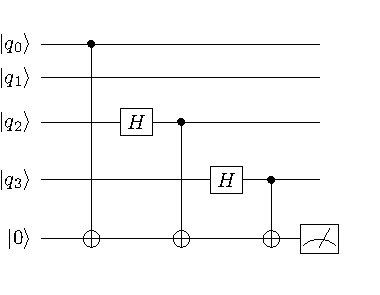
\includegraphics[width=0.4\textwidth]{Measurement}
\caption{Circuit used to measure the parity of a term given by $Z_0 \mathbf{1}_1 X_2 X_3$. The state beginning in the state $\ket{0}$ is the ancilla qubit. Note that this string does not occur in our Hamiltonian, it is purely illustrative.} \label{fig:m}
\end{figure}

After determining the expectation value at certain values of the parameters we want to optimize the parameters to find a minimum in the parameter space. For this report the Nalder-Mead algorithm was implemented to perform this optimization. A detailed description of this algorithm goes beyond the scope of this report, see for example Lagarias \textit{et al.} (1998) \cite{neldermead} for a further description. Important to note is that this algorithm has 4 parameters, which we call here $\rho$, $\chi$, $\gamma$ and $\sigma$, which control various steps of the algorithm. 


\subsection{Quantum Phase Estimation} \label{sec:qpe}

A different method to perform ground state preparation is by use of Quantum Phase Estimation (QPE). The QPE algorithm uses a series of a controlled version of the time evolution unitary $e^{- i H t}$. This unitary is applied to some initial state and controlled by a collection of $L$ ancilla qubits. This collection of ancillas is prepared in the $\ket{+}$ state. The repeated application of the unitary to our initial state projects it to a eigenstate of the unitary, and therefore of the Hamiltonian. In order to determine to which eigenstate the algorithm was projected we apply inverse QFT to our ancilla register and measure them. To use QPE to prepare the groundstate we use the algorithm and only keep the states where the ancilla register measures to the desired eigenstate.


\subsection{Time Evolution}

To study the time evolution from 0 to a time $t$ of our system given by Hamiltonian $H$ we need the unitary operator given by $U = e^{-iHt}$. In order to construct this unitary we use the first order Trotter approximation to write:

\begin{align*}
e^{-it \sum_j h_j \sigma_j } = \Pi_j e^{-it \sigma_j} + \hat{O}
\end{align*}

where the $\hat{O}$ operator denotes a error arrising from the non commutativity of Pauli strings which is of order 1 in this case. In order to visualize this error we look at the difference between time evolution by $e^{-i H t}$ and by $\Pi_j e^{-it \sigma_j}$. We do this by using numpy to calculate the exact\footnote{In general matrix exponentials are not exact since they are defined as a infinite (Taylor) series, but the approximation by numpy has a smaller error compared to the other elements in the experiment.} matrix exponential of both expressions, using those matrices to do time evolution and then look at their respective three body contact densities (as defined in section \ref{sec:modelback}). 


\begin{figure}[H]
\centering
\begin{subfigure}{.49\textwidth}
  \centering
  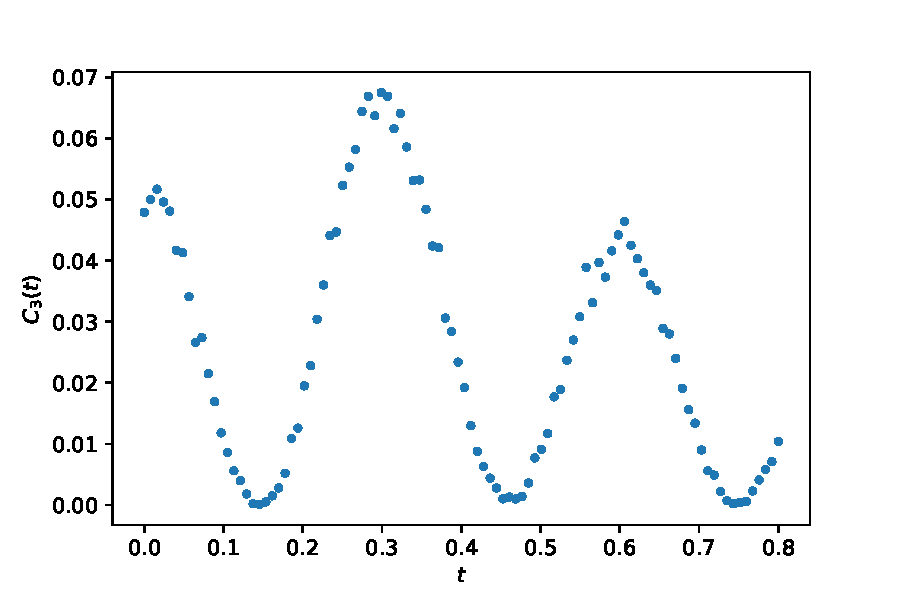
\includegraphics[width=\linewidth]{ExactSingle}
  \caption{Full exponential.}
  \label{fig:fullexp}
\end{subfigure}
\begin{subfigure}{.49\textwidth}
  \centering
  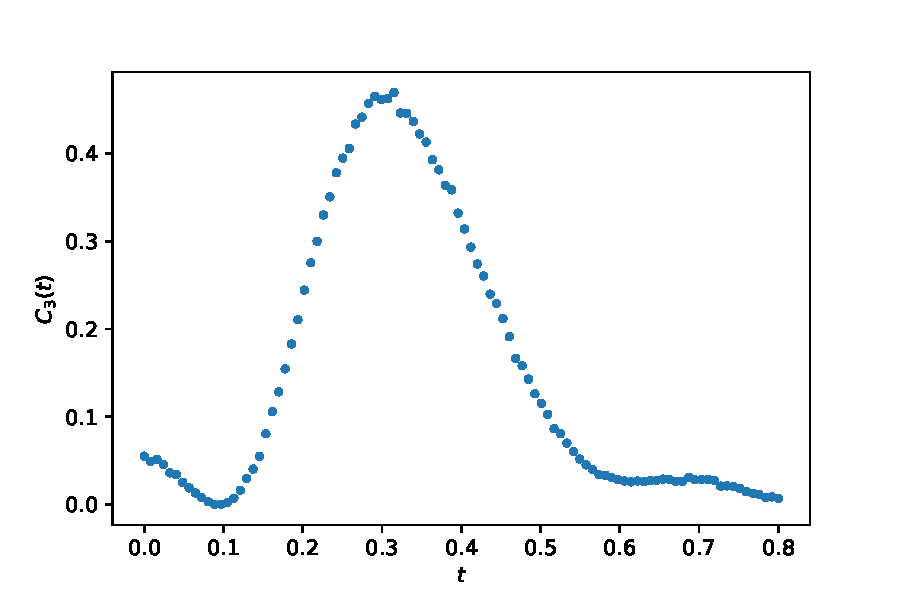
\includegraphics[width=\linewidth]{ExactProductSingle}
  \caption{Trotterized exponential.}
  \label{fig:sub2}
\end{subfigure}
\caption{Three body contact density for a initial state given by the ansatz given in figure \ref{fig:ansatz} with $\theta = 1.4$ and $\phi = 0.4$ under the time evolution under the Hamiltonian given by equation \ref{eqn:hamlimit} by: a) full matrix exponential and b) trotterized exponential.  Note the difference between y-axis ranges.}
\end{figure}



The trotterization however allows us to implement the time evolution using the simple gates we have access to on quantum computers. To reduce the error we can use multiple trotterization steps to arrive at the time $t$ by using:

\begin{align*}
e^{A+B} = \left[ \left[ e^{A+B} \right]^\frac{1}{k} \right]^k =\left[  e^{A/k+B/k} \right]^k = \left[  e^{A/k} e^{B/k} + O_k \right]^k
\end{align*}

where the error $O_k$ now scales as $O(||A|| \cdot ||B||/k^2)$. So when we use multiple trotter steps the error decreases.

\subsection{Sources of Error}

The VQE begins with a choice of an ansatz. Since it is not given that the chosen ansatz can represent the ground state there is an error from this difference. To optimize the VQE we need to determine the exception value of the Hamiltonian. This is done by repeatedly measuring the system and determining the average. In this averaging we have a statistical error. The optimization involves searching a parameter space for the lowest energy. In this search it is likely we will end up at some minimum other than the optimal minimum which also gives an error in the ground state estimation.
\\
\\
For the time evolution by we have the error due to the trotterization. For the determination of the three body contact density we also have statistical error in the estimation of the probability for the system to be in the state $\ket{0000}$.
\\
\\
Since our simulations are run at a finite machine precision we also have some error due to this but this error is probably far smaller than the other errors.

\subsection{Linear Response} \label{sec:linres}

An interesting extension to the system described above is to observe how it reacts to perturbations. We here follow the methods as described by Roggero \& Carlson (2018) \cite{linres}. We study how our system reacts to perturbations given by an operator $O$. We are interested in the Dynamical Response Function for this operator which is defined as:

\begin{align*}
S_O (\omega) = \sum_\nu |\bra{\psi_\nu} O \ket{\psi_0}|^2 \delta (E_\nu - E_0 - \omega)
\end{align*}

We estimate this function by using three unitary operators: $U_G$ which prepares the initial state, $U_O$ which implements time evolution under $O$ for a short time $\gamma$ en $U_t$ which implements time evolution under the Hamiltonian. We use these unitary operators and an ancilla qubit to prepare the system in a state $\ket{\psi_O} \sim O \ket{\psi_0}$. We can then use QPE as described above to extract the probabilities $|\bra{\psi_\nu} O \ket{\psi_0}|^2$ and use those to estimate $S_O (\omega)$.

\subsection{Implementation}

The quantum circuits as described in this report were implemented and simulated using cirq 0.8.0.dev \cite{cirq} where SymPy 1.5.1 \cite{sympy} was used for symbolic computations. Our implementation was benchmarked against implementations found in OpenFermion 0.11.0 and OpenFermion-Cirq 0.4.0.dev \cite{openfermion}. Plots were made using MatPlotLib 3.1.3 \cite{matplotlib}. To perform various numerical functions NumPy 1.18.1 \cite{numpy} was used.


\section{Results}

For all plots the averaging was performed using $10^4$ measurement samples unless stated otherwise.

\subsection{Ground State Preparation}

We first try to find a state close to the ground state by using the variational quantum eigensolver (VQE) algorithm as described in section \ref{sec:VQE}. We use the ansatz as postulated by Roggero \textit{et al.} (2019) \cite{neutscat} given in figure \ref{fig:ansatz}.

\begin{figure}[H]
\centering
	%\includegraphics[width=0.4\textwidth]{ansatz}
	\todo[inline]{Removed sourced image.}
\caption{Ansatz as used for the optimization with parameters $\theta$ and $\phi$. Source: \cite{neutscat}.} \label{fig:ansatz}
\end{figure}

We first start at the same values ($U = -7$, $V = 28$, $t = 1$) of the parameters in the Hamiltonian as used in \cite{neutscat}. We use the Nelder-Mead algorithms with parameters $\rho = 1$, $\chi = 2$, $\gamma = 1/2$ and $\sigma = 1/2$ for the optimization. Our implementation of the VQE algorithm finds a ground state energy given in table \ref{tab:results}. In this table we compare this value with the value found by the VQE as implemented in OpenFermion and with the exact ground state energy found using numpy.

\begin{table}[H]
\centering
\caption{Ground state energy as found using our implementation of the VQE and OpenFermion compared to the exact ground state energy.}
\begin{tabular}{|l|lll|}
\hline
                    & Implemented VQE & OpenFermion & Exact ground state \\ \hline
Ground state energy & -4.355          & -4.415      & -4.843             \\ \hline
\end{tabular} \label{tab:results}
\end{table}



To see how the difference between the ground state energy found using VQE and the exact ground state energy (further called $\Delta E$) varies for different values of $U$, $V$ and $t$ we apply the VQE at a range of values for those parameters. When we vary a parameter we keep the other two fixed at the values previously defined. We run the algorithm a number of times at each set of the parameters and pick the lowest found error to mitigate the problem of the optimization getting stuck in some local minimum.
\\
\\
In figure \ref{fig:uerror} we see the error for a range of $U$ values. We see that for postive values this error increases sharply.

\begin{figure}[H]
\centering
	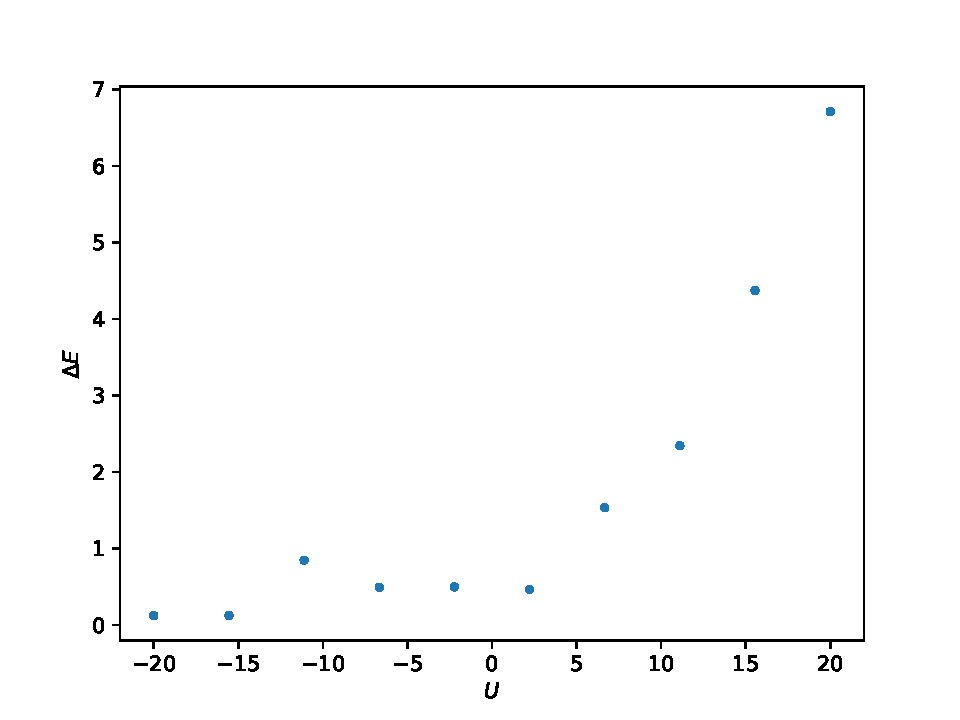
\includegraphics[width=0.7\textwidth]{uerror}
\caption{Difference between the lowest energy found by the VQE and the exact ground state energy at a range of values of the parameter $U$ with $V = 28$ and $t = 1$.} \label{fig:uerror}
\end{figure}

In figure \ref{fig:verror} we see the error for a range of $V$ values. We see again that for postive values this error increases sharply.

\begin{figure}[H]
\centering
	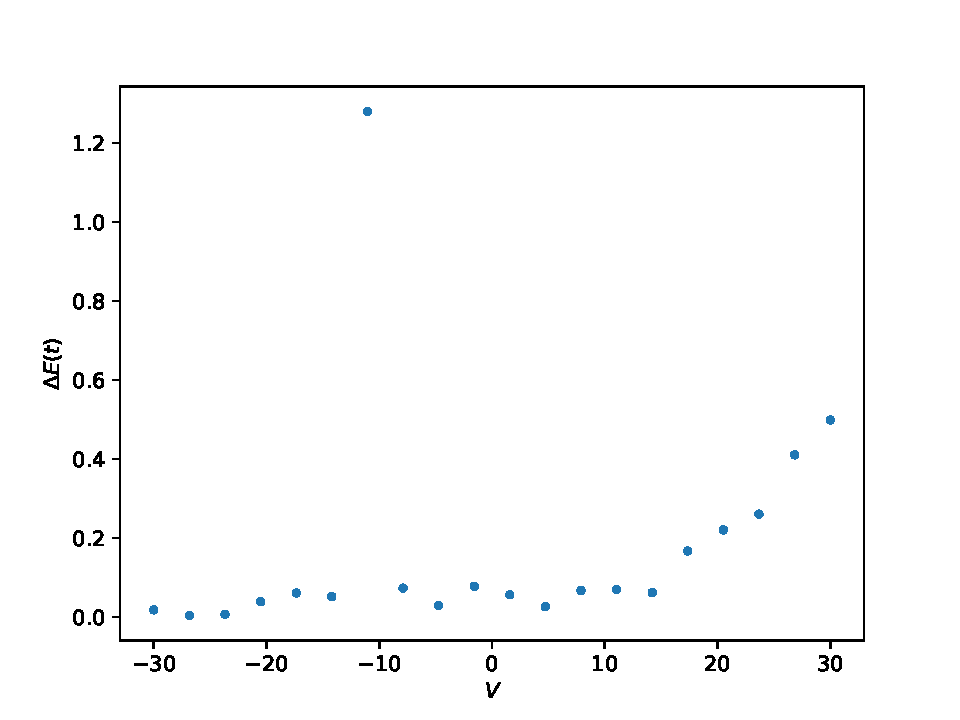
\includegraphics[width=0.7\textwidth]{verror}
\caption{Difference between the lowest energy found by the VQE and the exact ground state energy at a range of values of the parameter $V$ with $U = -7$ and $t = 1$. The outlier is probably a point where the optimizer got stuck in a local minimum.} \label{fig:verror}
\end{figure}


In figure \ref{fig:terror} we see the error for a range of $t$ values. We see that the error peaks around $t = 0$ and decreases for increasing $|t|$.

\begin{figure}[H]
\centering
	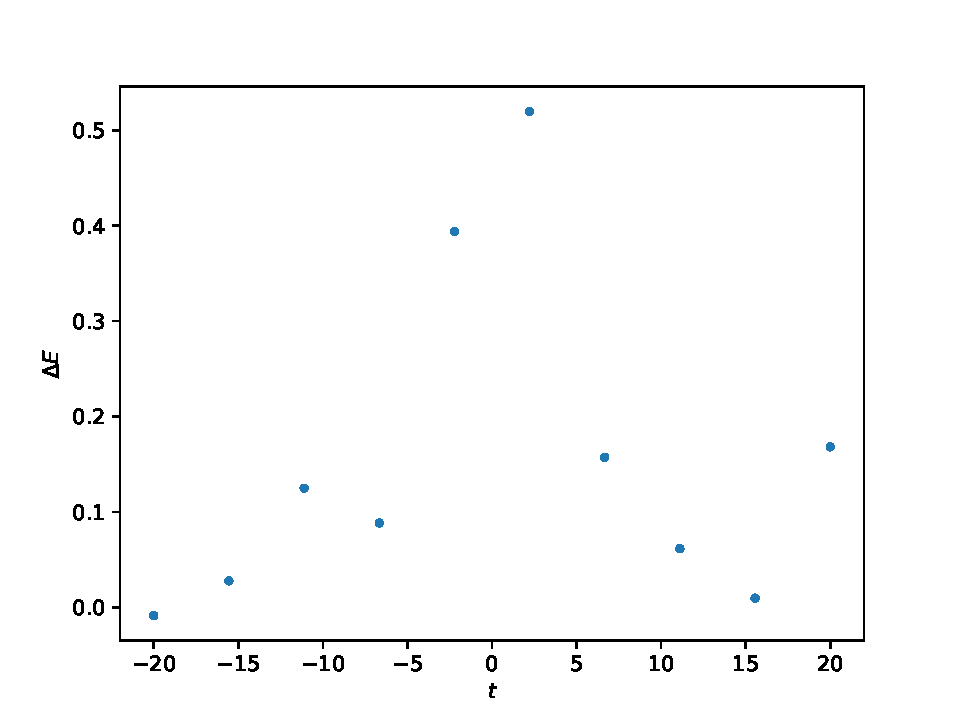
\includegraphics[width=0.7\textwidth]{terror}
\caption{Difference between the lowest energy found by the VQE and the exact ground state energy at a range of values of the parameter $t$ with $V = 28$ and $U = -7$. The error peaks around $t = 0$ and tends towards as zero as $|t|$ in increases.} \label{fig:terror}
\end{figure}


We can also use Quantum Phase Estimation (QPE) to prepare a groundstate. We do this by applying the algorithm as described in section \ref{sec:qpe}. We start from the ansatz as given in figure with the parameters as found by the VQE. In figure \ref{fig:qpe} we see a histogram for the phase as determined by measuring the ancilla qubits. We see that our QPE projects a fraction of our runs to the ground state (given by the blue line in the figure).

\begin{figure}[H]
\centering
	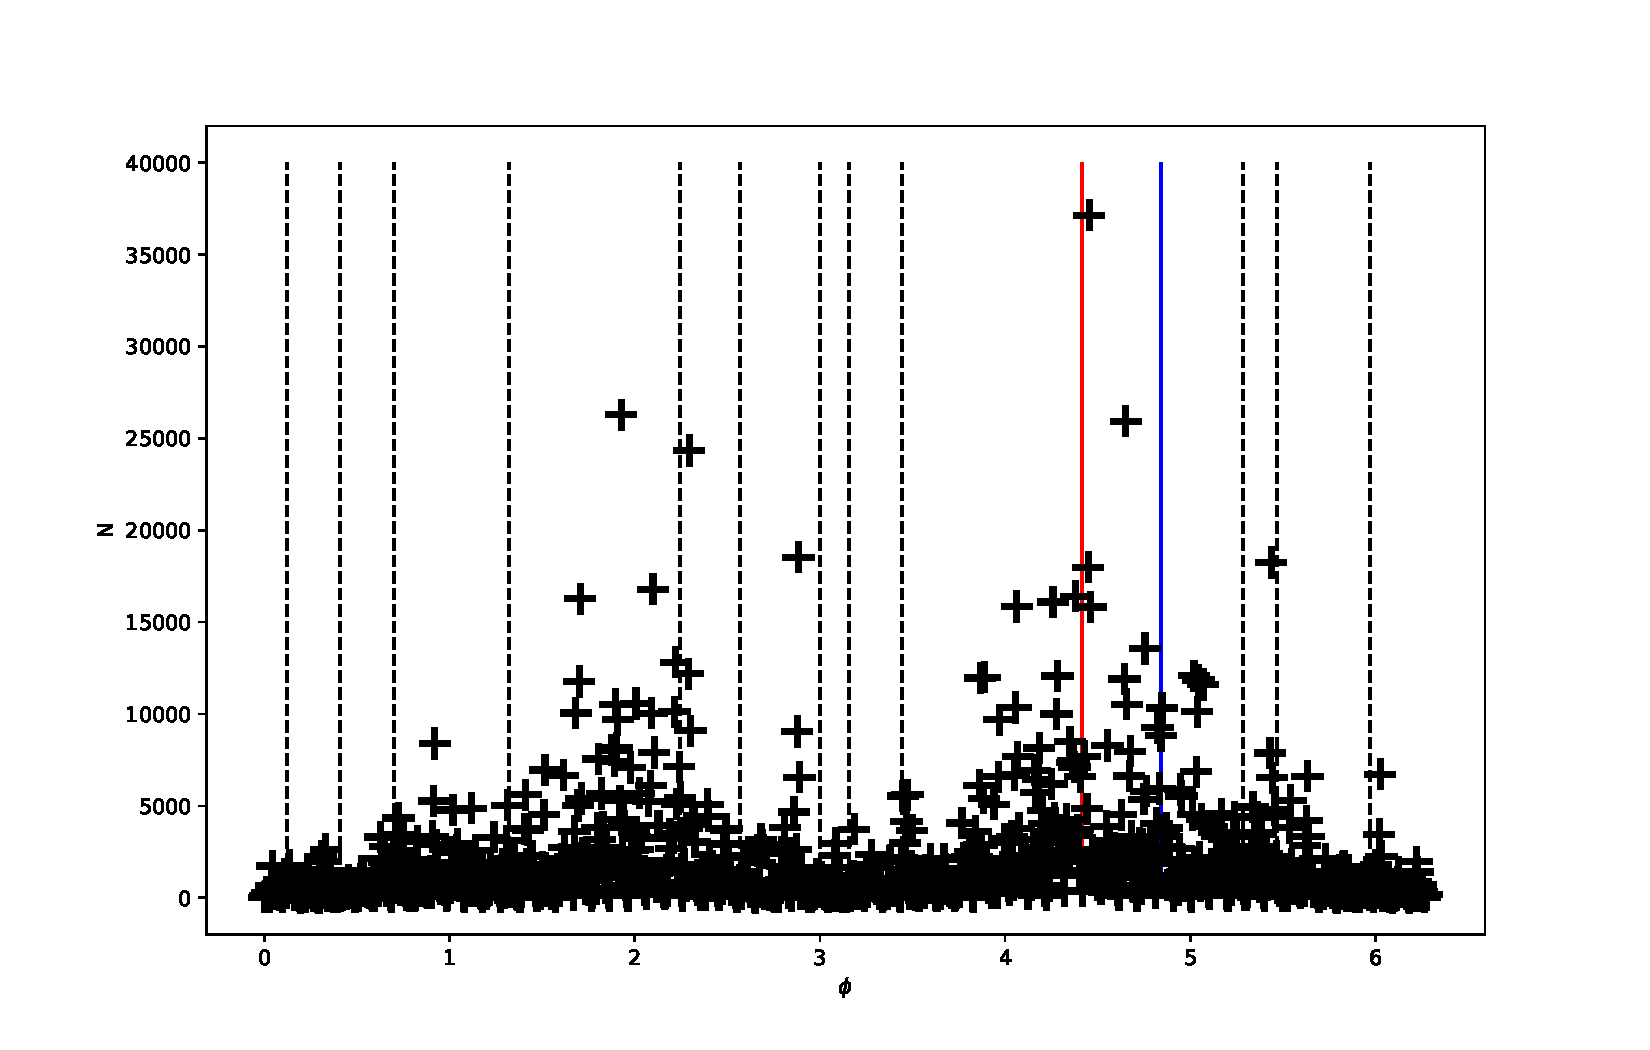
\includegraphics[width=\linewidth]{qpe}
\caption{Histogram of the ancilla measurements for the QPE algorithm for our Hamiltonian for $L = 10$ ancillas. The dashed black lines denote eigenvalues of the Hamiltonian, the red blue line denotes the lowest eigenvalue and the red line denotes the energy as found using the VQE algorihtm.} \label{fig:qpe}
\end{figure}



\subsection{Time Evolution}

In order to evaluate the time evolution of the model we look at the three body contact density as defined in section \ref{sec:modelback}. We begin by looking at the time evolution by a single trotter step with the initial state as found by the VQE, this is given in figure \ref{fig:tbc1}. We see that our results are consistent with the result found by Roggero \textit{et al.} (2019) \cite{neutscat}.

\begin{figure}[H]
\centering
	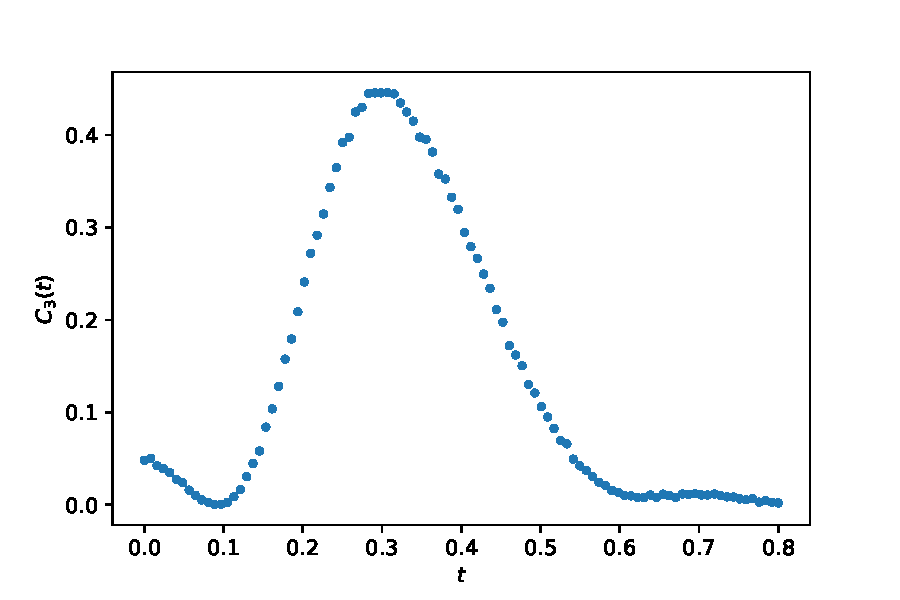
\includegraphics[width=0.7\textwidth]{ThreeBodyContactGates1}
\caption{Three body contact density as a function of time. Time evolution performed using a single trotter step per time point.} \label{fig:tbc1}
\end{figure}

When increasing the number of trotter steps we use we see that the plot behaviour changes drastically (figure \ref{fig:tbc2}). We see that for increasing number of trotter steps the behaviour approaches that of the exact exponential as given in figure \ref{fig:fullexp}. Which is expected since the error due to trotterization should decrease with additional trotter steps.

\begin{figure}[H]
\centering
\begin{subfigure}{.32\textwidth}
  \centering
  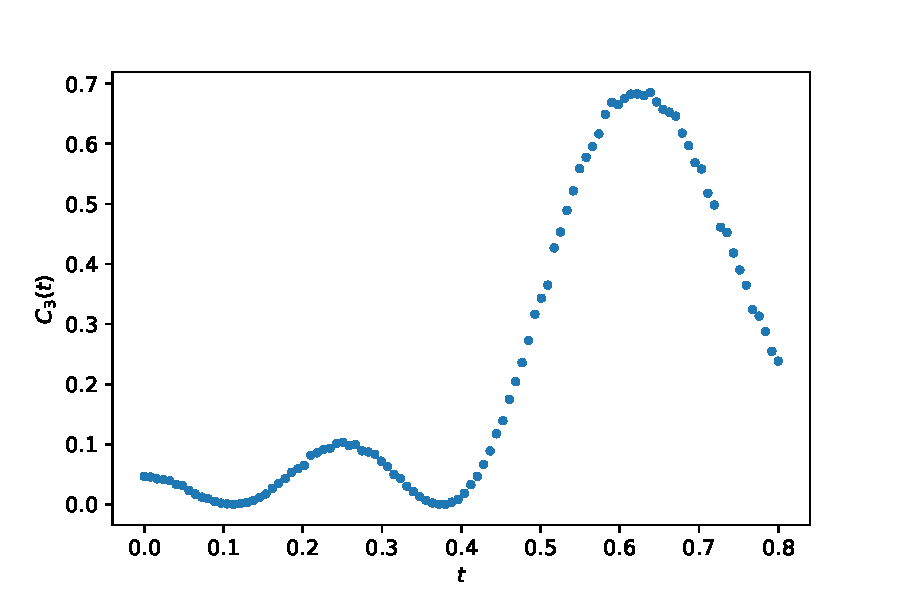
\includegraphics[width=\linewidth]{ThreeBodyContactGates2}
  \caption{2 steps.}
  \label{fig:sub1}
\end{subfigure}
\begin{subfigure}{.32\textwidth}
  \centering
  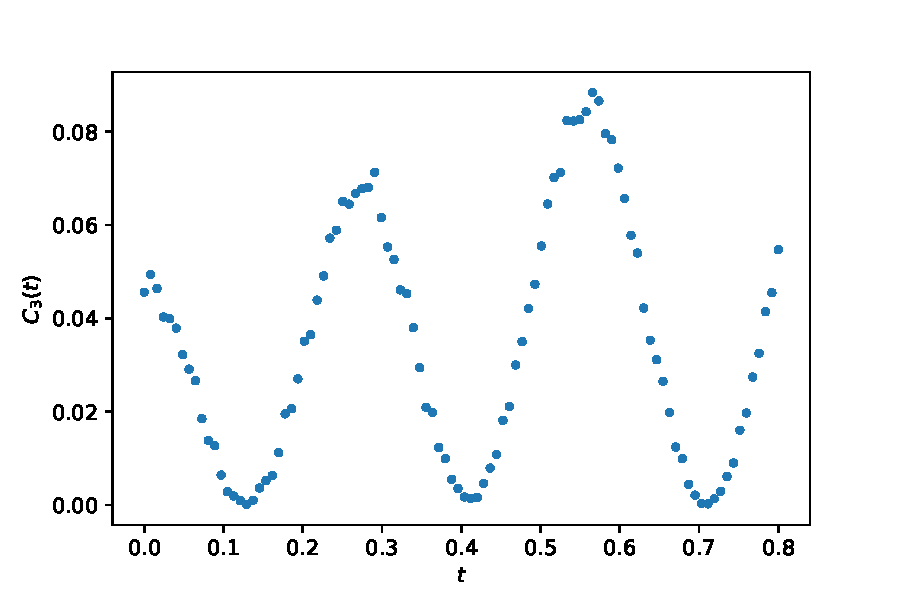
\includegraphics[width=\linewidth]{ThreeBodyContactGates5}
  \caption{5 steps.}
  \label{fig:sub2}
\end{subfigure}
\begin{subfigure}{.32\textwidth}
  \centering
  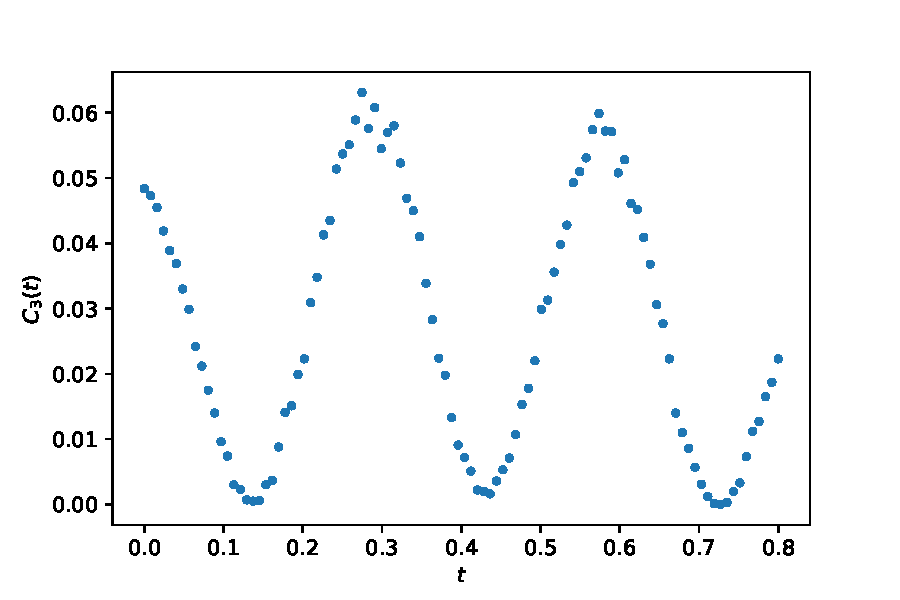
\includegraphics[width=\linewidth]{ThreeBodyContactGates10}
  \caption{10 steps.}
  \label{fig:sub3}
\end{subfigure}
\caption{Three body contact density as a function of time. Time evolution performed using a) 2, b) 5, c) 10, trotter steps per time point.} \label{fig:tbc2}
\end{figure}

We can also look at time evolution with a state we prepared using QPE, first using a single trotter step. This is given in figure \ref{fig:qpetbc1}.
We see that this result differs from the result using the VQE, which gives an indication that it prepared a different initial state.
\begin{figure}[H]
\centering
	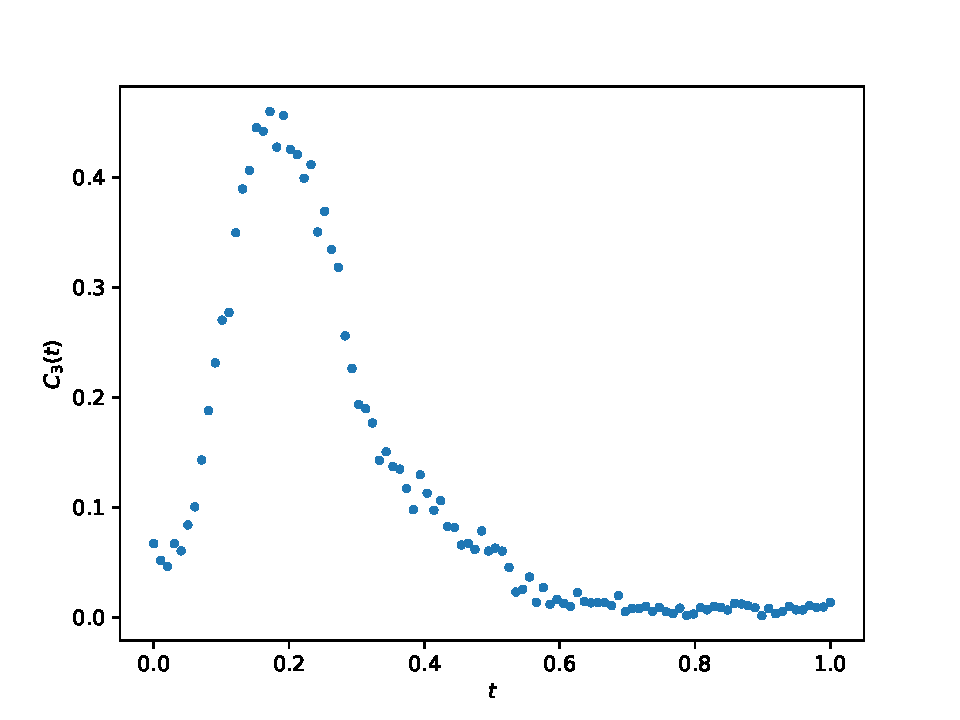
\includegraphics[width=0.7\linewidth]{QPEtbc1}
\caption{Three body contact density as a function of time for a state initialised using QPE. Time evolution performed using a single trotter step per time point. } \label{fig:qpetbc1}
\end{figure}

For 10 trotter steps this result is given in figure \ref{fig:qpetbc10}. 

\begin{figure}[H]
\centering
	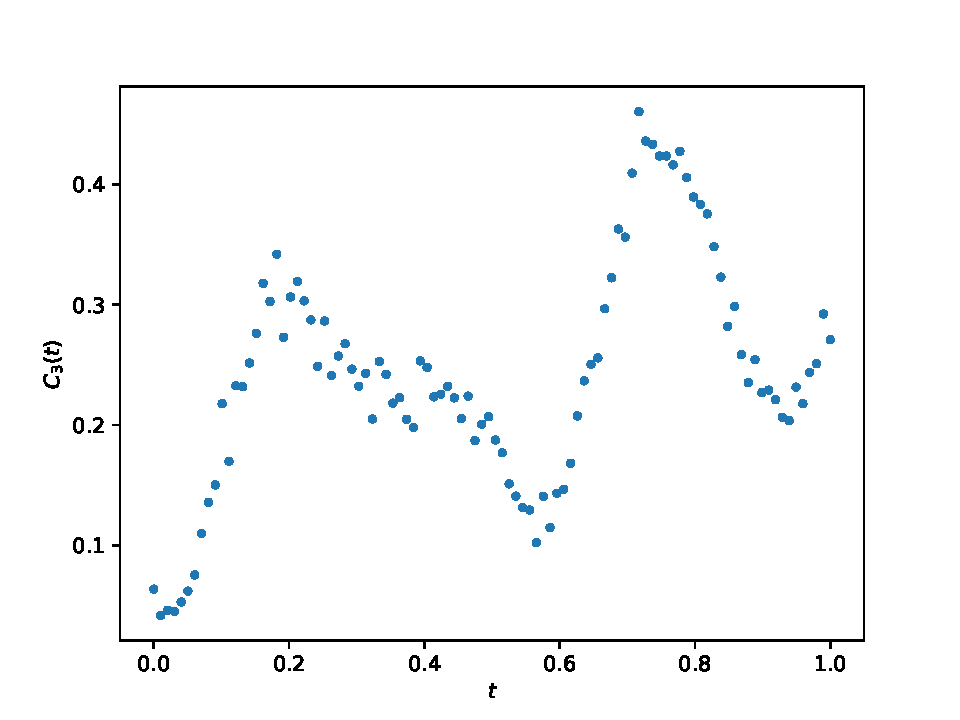
\includegraphics[width=0.7\linewidth]{QPEtbc10}
\caption{Three body contact density as a function of time for a state initialised using QPE. Time evolution performed using 10 trotter steps per time point.}  \label{fig:qpetbc10}
\end{figure}

\subsection{Linear Response}

For the linear response we only have some preliminary results.
\\
\\
We look at perturbations given by $O = Z_3$ and apply the algorithm as described in section \ref{sec:linres} and by Roggero \& Carlson (2018) \cite{linres}. We have $\gamma = 0.1$ and use the same parameters in the Hamiltonian as described above. We get an estimation of $S_O(\omega)$ given in figure \ref{fig:SO}. We see that the rough structure seems to be similar to that in \cite{linres} however there are mainly disagreements. Due to time constraint we weren't able to improve results.

\begin{figure}[H]
\centering
	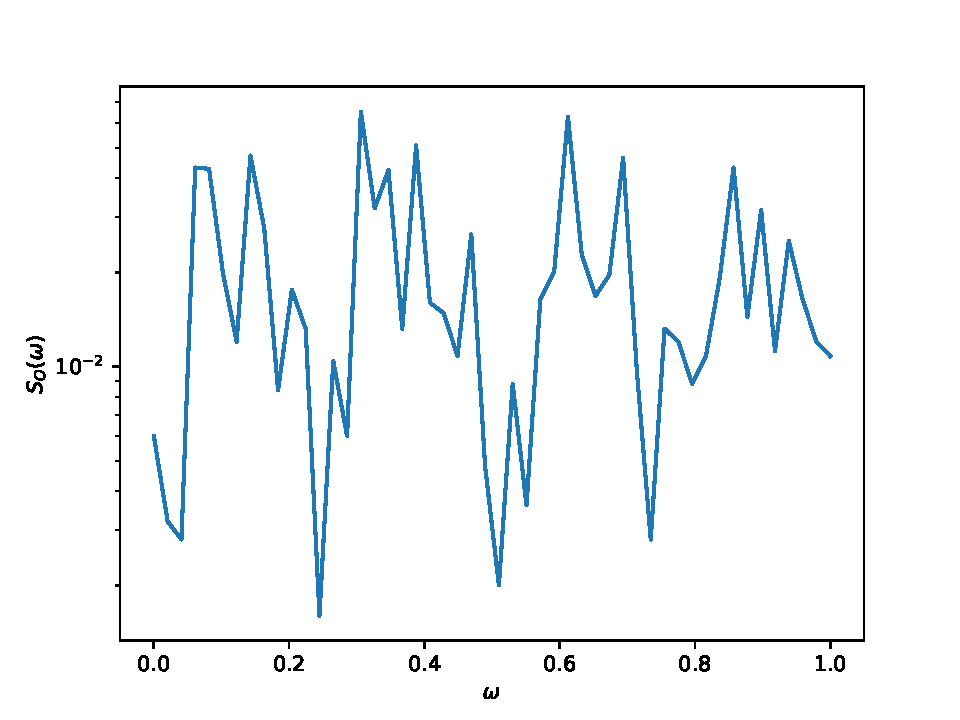
\includegraphics[width=0.7\linewidth]{SO}
\caption{Estimation of the response function $S_O(\omega)$. The rough structure seems to be consistent with expectations.}  \label{fig:SO}
\end{figure}

\section{Conclusion}

We implemented the triton toy model as defined by Roggero \textit{et al.} (2019) \cite{neutscat} and approximated the ground state using the variational quantum eigensolver (VQE) and qunatum phase estimation (QPE) algorithm. Using the VQE we found a ground state energy approximation consistent with the results found in \cite{neutscat} and with the results found using the VQE as implemented in OpenFermion.
\\
\\
When looking at the time evolution using a single trotter step we found results consistent with \cite{neutscat}. When implementing time evolution with multiple trotter steps we find different results that do match with results using exact matrix exponentials using numpy.

\begin{thebibliography}{99}
\bibitem{neutscat} Alessandro Roggero, Andy C.Y. Li, Joseph Carlson, Rajan Gupta \& Gabriel N. Perdue (2019), \textit{Quantum Computing for Neutrino-nucleus Scattering}, Preprint at \url{https://arxiv.org/abs/1911.06368}.

\bibitem{neldermead} Jeffrey C. Lagarias, James A. Reeds, Margaret H. Wright \& Paul E. Wright (1998), \textit{Convergence Properties of the Nelder--Mead Simplex Method in Low Dimensions}, SIAM J. Optim., 9(1), 112–147.

\bibitem{linres} Alessandro Roggero \& Joseph Carslon (2019), \textit{Dynamic linear response quantum algorithm}, PHYSICAL REVIEW C 100, 034610.

\bibitem{cirq} The Cirq Devolopers, \textit{Cirq, A python framework for creating, editing, and invoking Noisy Intermediate Scale Quantum (NISQ) circuits}, \url{https://github.com/quantumlib/Cirq}.

\bibitem{sympy} Aaron Meurer​, Christopher P. Smith, Mateusz Paprocki, Ondrej Certik, Sergey B. Kirpichev, Matthew Rocklin, AMiT Kumar, Sergiu Ivanov, Jason K. Moore, Sartaj Singh, Thilina Rathnayake, Sean Vig, Brian E. Granger, Richard P. Muller, Francesco Bonazzi, Harsh Gupta, Shivam Vats, Fredrik Johansson, Fabian Pedregosa, Matthew J. Curry, Andy R. Terrel, Stepan Roucka, Ashutosh Saboo, Isuru Fernando, Sumith Kulal, Robert Cimrman \& Anthony Scopatz (2017), \textit{SymPy: symbolic computing in Python},  PeerJ Computer Science 3:e103.

\bibitem{openfermion} Jarrod R. McClean, Kevin J. Sung, Ian D. Kivlichan, Xavier Bonet-Monroig, Yudong Cao, Chengyu Dai, E. Schuyler Fried, Craig Gidney, Brendan Gimby, Pranav Gokhale, Thomas Häner, Tarini Hardikar, Vojtĕch Havlíček, Oscar Higgott, Cupjin Huang, Josh Izaac, Zhang Jiang, William Kirby, Xinle Liu, Sam McArdle, Matthew Neeley, Thomas O'Brien, Bryan O'Gorman, Isil Ozfidan, Maxwell D. Radin, Jhonathan Romero, Nicholas Rubin, Nicolas P. D. Sawaya, Kanav Setia, Sukin Sim, Damian S. Steiger, Mark Steudtner, Qiming Sun, Wei Sun, Daochen Wang, Fang Zhang \& Ryan Babbush (2017), \textit{OpenFermion: The Electronic Structure Package for Quantum Computers}, Preprint at \url{https://arxiv.org/abs/1710.07629}.


\bibitem{matplotlib} John D. Hunter (2007), \textit{Matplotlib: A 2D Graphics Environment}, Computing in Science \& Engineering, 9, 90-95.

\bibitem{numpy} Travis E. Oliphant (2006), \textit{A guide to NumPy}, Trelgol Publishing, USA.





%\bibitem{accvqe} D. Wang, O. Higgott \& S. Brierley (2019), \textit{Accelerated Variational Quantum Eigensolver}, Phys. Rev. Lett. 122, 140504.
%https://arxiv.org/pdf/1802.00171.pdf

%\bibitem{hamavg} J. Romero \textit{et al.} (2018), \textit{Strategies for quantum computing molecular energies using the unitary coupled cluster ansatz}, Quantum Sci. Technol. 4 014008.
%https://arxiv.org/pdf/1701.02691.pdf
\end{thebibliography}


%https://docs.microsoft.com/en-us/quantum/concepts/pauli-measurements?view=qsharp-preview
%https://pure.tue.nl/ws/portalfiles/portal/147595552/Bogaarts_T.J._1000549_BEP_verslag.pdf



\include{appendix}

\end{document}